\documentclass[9pt,twocolumn,twoside,lineno]{style}

\articletype{NEI} % article type

\title{Resenhas 05: \textit{Institutions, Contracts and Organizations: Perspectives from New Institutional Economics} (Menárd 2000)}
\date{08 de maio de  2020}

\author[$\ddagger$]{Gabriel Petrini}

\affil[$\ddagger$]{Doutorando no instituto de Economia da Unicamp}

\keywords{Keyword \\ Keyword2 \\ Keyword3 \\ ...}

\runningtitle{Resenhas 05} % For use in the footer 

%% For the footnote.
\runningauthor{Petrini}

\begin{abstract}
\end{abstract}

\begin{document}

\maketitle\articletypemark
\marginmark
\thispagestyle{firststyle}
\section*{Benham \& Benham: Measuring the costs of exchange}

\subsection*{Introdução}

Os autores iniciam o capítulo pontuando que os custos de transação são o principal conjunto de preços da economia, mas pouco se sabe sobre sua mensuração e variação.
Em seguida, definem custos de transação como \textbf{custos de oportunidade} que os agentes econômicos incorrem quando recorrem à uma forma de troca para obter um ativo específico dada uma configuração institucional.

\subsection*{Elementos dos custos de transação}

Os autores ressaltam que existem poucos estudos que estimam os custos de transação e que mesmos estes são pouco comparáveis. Dentre os motivos, pontuam a ausência de consenso na definição do termo. Partindo da contribuição de Furubotn e Reichter, elencam duas variantes dos custos de transação: (i) fixos e (ii) variáveis. Os primeiros estão associados à investimentos específicos em um dado arranjo institucional enquanto os segundos dependem do número ou do volume das transações.
Além disso, afirmam que os custos de produção e de transação são definidos \textbf{conjuntamente} e, portanto, existem dificuldades em separá-los. Também pontuam que se os custos de transação são muito elevados, muitas das transações associadas deixariam de ocorrer. Argumentam que a lei do preço único não se aplica também uma vez que indivíduos de uma mesma sociedade podem ter custos de transação distintos.

\subsection*{Custos de troca}

Os autores propõem analisar um subconjunto de custos de transação: custos de troca. Definem este conceito como o custo de oportunidade de todos os recursos (tempo, dinheiro e bens) de um indivíduo $i$ usar uma troca $j$ para obter um bem $k$ em um arranjo institucional $m$ ($C_{ijkm}$). Sendo assim, os custos de troca são a soma dos custos de produção e de transações específicas incorridas por um agente. Uma vez que não é possível decompor os custos diretamente em seu equivalente em produção e transação, irão adotar uma \textbf{análise comparativa}. Em outros termos, esta proposta enfatiza os custos de oportunidade que um indivíduo incorre ao estabelecer uma troca específica em uma dada especificidade institucional.
Para tanto, os autores precisam padronizar a metodologia adotada. Dentre as dificuldades, afirmam que os preços de mercado não refletem bem os custos de oportunidade. Sendo assim, optam por analisar os bens intermediários.

\subsection*{Estudos de casos}

Nesta seção, os autores apresentam alguns estudos de caso, são eles:

\begin{description}
	\item[Telefonia] Os custos de troca associados ao setor de telefonia determinam o tamanho das redes de comunicação, tamanho do mercado e grau de especialização. O estudo foca no custos de obtenção de um telefone comercial em que investigam os custos de transferência de propriedade.
	\item[Novo negócio] São investigados os custos associados a criação de um novo negócio em que foram calculados os custos em dias para conseguir os requerimentos necessários para tal. Relatam casos em que o tempo para conseguir iniciar um novo negócio é consideravelmente maior na ausência de contatos influentes.
	\item[Fronteiras nacionais] Argumenta que as transações transfronteiriças são um indicador do tamanho do mercado de uma economia. Para tanto, calculam o tempo de espera para escoar os produtos no porto.
\end{description}
Os estudos ilustrados anteriormente indicam que a \textbf{variação} dos custos de troca são enormes e que os custos de oportunidade associados à obtenção de um bem são bastante distintos dos preços de mercado.

\subsection*{Pesquisas futuras}

Os autores argumentam que o retorno desta agenda de pesquisa será maior quanto maior os esforços coletivos entre diferentes países. Além disso, os casos apresentados ilustram que esta metodologia é factível enquanto a variedade dos resultados indicam a importância de se estudar tais custos. Em seguida, afirmam algo semelhante às vantagens comparativas em que pontuam que se os custos de troca de um país forem consideravelmente maiores em um país do que em outro, é esperado que o país que apresente maiores custos não produza o bem em questão. Por outro lado, se os custos de oportunidade são menores, as transações podem em distâncias maiores e por períodos mais longos. Encerram afirmando que estar diferenças dependem do grau de especialização e do desempenho da economia.
\section*{Brousseau e Fares: \textit{Incomplete contracts and governance structures: are incomplete contract theory and new institutional economics substitutes or complements?}}

\subsection*{Introdução}

Ao longo deste capítulo, os autores investigam as diferenças e compatibilidades da Teoria dos Contratos Incompletos (TCI) com a Nova Economia Institucional (NEI). Dado que esta última corrente tem sido analisada no decorrer da disciplina, será descrita em menor detalhe. Dito isso, cabe mencionar que a TCI se propõe a explicar os mecanismos de coordenação verticais dentro do aparato neoclássico. Além disso, as hipóteses racionais e cognitivas da TCI se diferem das da NEI uma vez que a primeira supõe racionalidade limitada apenas na instância que avalia e \textbf{executa os contratos}. Outra diferença é que a TCI analisa tipos de contratos que podem ser implementados em uma dada estrutura institucional.

\subsection*{Teoria dos contratos incompletos: análise dos impactos das instituições sobre os contratos}

\subsubsection*{Fundadores da TCI}

Os autores apresentam o modelo Grossman e Hart (G\&H) em que uma integração vertical mitiga (mas não suprime) o problema de espera e sub-investimento decorrente da incompletude dos contratos. Este modelo possui duas hipóteses principais: investimentos específicos não são-contratáveis dados os elevados custos de elaboração dos contratos; as variáveis relevantes para a relação contratual não são verificáveis por terceiro e, assim, não contratáveis. Em seguida, os autores explicitam o modelo formalmente comparando o resultado ótimo com o sub-ótimo em que há sub-investimento. Tal resultado decorre dos problemas de espera uma vez que as partes temem (\textit{ex ante}) uma desapropriação \textit{ex post}. Com a integração vertical, uma das partes investe em seu nível ótimo e, assim, captura todo o excedente \textit{ex post}.
Críticas ao modelo apontavam para a tensão entre as hipóteses de racionalidade substantiva entre as partes envolvidas junto da racionalidade limitada  para justificar os custos de elaboração contratual (Tirole 1999). Como resposta, surgiram modelos que parte da não-verificabilidade de todas as informações de uma das partes.

\subsubsection*{TCI e os aspectos de inverificabilidade}

Um aprimoramento do modelo G\&H é o desenvolvido por Hart e Moore (H\&M) em que os autores  defende que os contratos são incompletos por: (i) incapacidade do avaliador (juiz) verificar o estado da natureza; (ii) incapacidade de ambas as partes evitarem renegociações \textit{ex post}. Em linhas gerais, há sub-investimento por conta do juiz não ser capaz de executar níveis ótimos de transação. Sendo assim, o problema da inverificabilidade pela escolha de uma classe particular de contratos. Em resumo, a principal hipótese recai sobre o nível de verificabilidade do juiz. 
Em seguida, os autores comparam o modelo H\&M com os de Aghion (ADR) para indicar  que os resultados são sensíveis ao grau de verificabilidade do juiz. Em particular, os resultados do modelo são sensíveis à alocação do poder de barganha entre as partes e garantias do \textit{status quo} que incentivam a investir. Caso o poder de barganha seja todo alocado para uma das partes, o problema de espera pode ser resolvido.

\subsubsection*{Crítica de Tirole e limitações analíticas da TCI}

Tirole rejeita que a incompletude contratual seja endogeneizada pela hipótese de não-verificabilidade. Em particular, rejeita a ideia de que a incompletude dos contratos por conta da hipótese de informações observáveis, mas não verificáveis uma vez que as partes sempre poderiam completar os contratos ao implementar um mecanismo de revelação que faça com que esta informação se torne verificável ao juiz.
No entanto, alguns autores argumentam que este mecanismo de Tirole tem limitações por requerer a implementação de penalidades elevadas junto de compromissos críveis. Em seguida, os autores pontuam as questões de \textbf{inconsistência lógica} da TCI e que a hipótese de não-verificabilidade é \textit{ad hoc} porque a estrutura institucional (juiz) que executa os contratos continua exógena. Isso decorre porque o juiz não é a única parte envolvida no processo contratual que possui racionalidade limitada.
Diferentemente da TCI, a NEI endogeniza as instituições. Além disso, as imperfeições de cada mecanismos de coordenação na NEI são reduzias quando realizados conjuntamente. Em outras palavras, a diversidade dos mecanismos de governança garantem que os agentes desempenhem coordenações a um custo menor.

\subsection*{Incompletude contratual e institucional na NEI}

\subsubsection*{Causas da incompletude: Racionalidade limitada e incerteza fundamental}

Em linhas gerais, a hipótese de racionalidade limitada na NEI não se restringe aos juízes e se estende para todos os agentes. Sendo assim, ao assumir que as tomadas de decisão levam tempo e são custosas, os agentes podem errar e estão sujeitos à assimetrias de informação. A outra razão da incompletude dos contratos é a existência de incerteza fundamental e, assim, não são capazes de estabelecer contratos contingenciais que encobrem todas as possibilidades futuras eficientemente.

\subsubsection*{Natureza intrínseca das estruturas de governança: Autoridade e execução}

Invés de elaborar contratos que lidem com todas as contingências \textit{ex ante}, elaboram mecanismos de decisão \textbf{\textit{ex post}} que indicam comportamentos necessários para os contratantes assegurarem a coordenação de forma eficiente e garantir a execução dos compromissos assumidos. Esses mecanismos de decisão se baseiam no reconhecimento de uma autoridade pelos contratantes e pelo princípio de subordinação. A divisão destas funções entre as partes é diferente em cada estrutura de governança. Tais mecanismos, no entanto, são insuficientes para garantir a coordenação. Em outras palavras, regras e ordens devem ser executadas para garantir a credibilidade dos compromissos contratuais. Ou ainda,  a incompletude dos contratos  implementa um mecanismo de autoridade. Como consequência, além das limitações do sistema legal, a incompletude dos contratos \textbf{\textit{per se}} gera questões de execução e, por conta disso, os agentes econômicos devem implementar mecanismos de auto-execução nas estruturas de governança que elaboram. Esta auto-execução depende da implementação de três classes de mecanismos:

\begin{itemize}
	\item Esquema de incentivo e coerção
	\item Mecanismos de supervisão
	\item Mecanismos de arbitragem para resolução de conflitos
\end{itemize}
Em resumo, estruturas de governança articulam mecanismos de atuação que as partes devem tomar para obterem coordenação de forma eficaz e as classes mencionadas anteriormente para assegurar a auto-execução de arranjos contratuais.

\subsubsection*{Articulação entre estruturas de governança coletivas e entre indivíduos}

Estruturas de governança intra-individuais (EGI) são elaboradas pelos agentes para completar as obrigações contratuais \textit{ex ante} e assegurar a auto-execução. Tais EGIs são desempenhadas em um nível bidirecional entre indivíduos e instituições coletivas. Em resumo, ambas são formas complementares de coordenação em que os agentes ajustam as vantagens de cada uma para reduzir os custos de transação. Quando uma EGI é desenhada, o comportamento dos agentes econômicos é restringindo pelos mecanismos institucionais \textit{ex ante}.

A NEI enfatiza que as governanças coletivas são executadas por instituições completas e incompletas uma vez que são elaboradas para desempenhar uma interação econômica de governança de forma não-intencional; são elaboradas por agentes que possuem racionalidade limitada; e a partir de um denominador comum dado pelos conjuntos de transação. Como consequência, algumas estruturas de governança devem ser desenvolvidas ao nível inter-individual na tentativa de completar a incompletude das governanças coletivas.

\subsubsection*{Endogeinização de sistemas de governança complexos}

Uma vez que o arranjo institucional é imperfeito e incompleto, os agentes precisam implementar EGI para obter coordenação. No entanto, também podem participar da elaboração de estruturas de governança coletivas. Sendo assim, as EGIs podem moldar a matriz institucional e aprimorá-la. Estes mecanismos de decisão completam a incompletude das regras e garantem que são executadas. Sendo assim, instituições são combinações de regras e instituições organizacionais. Os autores também pontuam que as instituições privadas devem ser comparadas com as públicas. Argumentam que quando os agentes precisam resolver um problema de coordenação, deve escolher reduzir custos de transação privados quando coordenam por meio de um mecanismo coletivo. Uma vez que os agentes não podem impactar as instituições públicas diretamente, devem criar voluntariamente uma estrutura coletiva privada especializada de modo a obter formas mais eficientes de coordenação coletiva. O trecho a seguir resume esta discussão (p.~ 416):

\begin{quote}
	In sum, economic agents have the possibility of assigning the various governance tasks to various entities according to the respective nature of the tasks and the ability of the entities. This enables them to play on the complementarities among public institutions, private institutions and inter-individual governance structuresto try to obtain the lowest possible transaction costs. NIE is thus able to explain the co-genesis and the joint properties of interindividual (contractual) governance structures and institutions (collective governance structures)
\end{quote}


\subsection*{Conclusão}

A incompletude dos contratos na TCI decorre da racionalidade limitada da personificação da estrutura institucional (juiz) e que os diferentes níveis de racionalidade deste juiz determinam os mecanismos de implementação das negociações. Na NEI, a incompletude dos contratos é resultado da racionalidade limitada de todos agentes econômicos. Além disso, as instituições não são exógenas e são elaboradas de forma imperfeita de modo que não conseguem zeras os custos de transação. Os agentes tentam escolher estruturas de governança complementares para reduzir tais custos. Sendo assim, a principal questão da NEI é comparar os custos relativos gerados pela combinação de vários mecanismos de coordenação. Em resumo, concluem que a TCI e a NEI são mais complementares do que excludentes uma vez que tratam de temas distintos. A TCI pode ser criticada por sua inconsistência lógica ou pelas hipóteses \textit{ad hoc}. A NEI, por outro lado, possui grandes dificuldades metodológicas apesar de possuir uma consistência interna elevada. Segue uma tabela que compara ambas abordagens.

\begin{figure}[h]
	\centering
	\caption{Resumo da comparação entre TCI e NEI}
	\label{fig:screenshot001}
	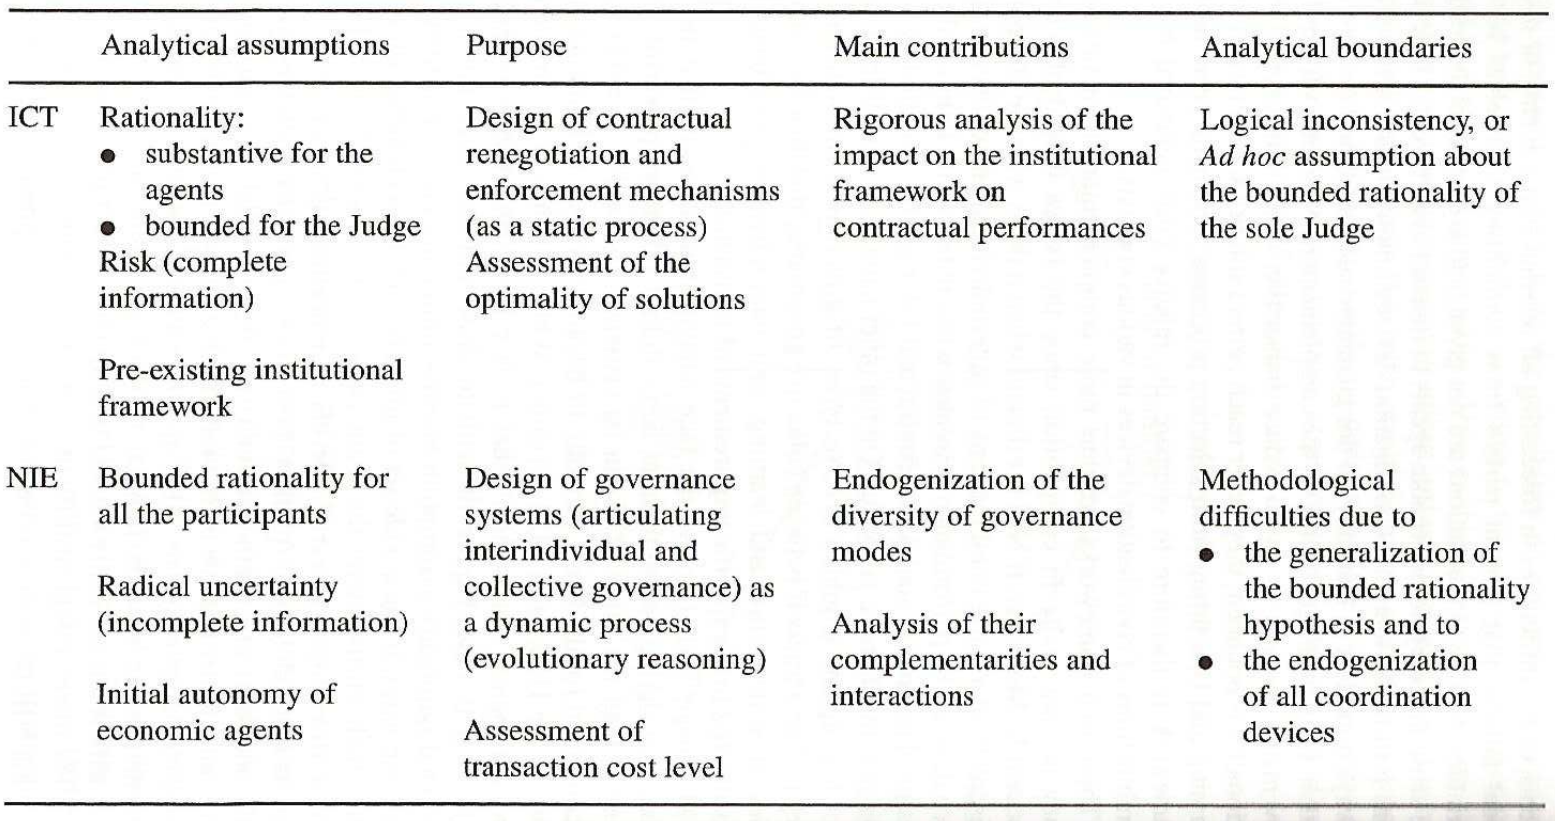
\includegraphics[width=\linewidth]{screenshot001}
\end{figure}



\begin{sigstatement}
	\sffamily
	\mdfdefinestyle{stylesigstyle}{linewidth=0.7pt,
		backgroundcolor=styleblueback,linecolor=stylebluetext,
		fontcolor=stylebluetext,innertopmargin=6pt,innerrightmargin=6pt,
		innerbottommargin=6pt,innerleftmargin=6pt}
	{%	
		\begin{mdframed}[style=stylesigstyle]%
			\section*{Dúvidas}%
	Ao proporem uma forma de mensuração dos custos de transação em uma perspectiva comparada, Benham e Benham (2000) tentam calcular os custos de ``troca'' incorridos por um agente em uma dada especificidade institucional. No entanto, supor que a estrutura institucional é dada não contraria as propostas da NEI em que as estruturas de governança são endógenas?
	
	Ao fim do capítulo, Benham e Benham (2000, p.~373) afirmam:
	
	\begin{quotation}
		If the price of an intermediate good neededfora final
		productis ten times higher in country A than in country B, we should not be
		surprised if country A does not producethatfinal product.
	\end{quotation}
	Seria essa um retorno das vantagens comparativas em uma nova roupagem teórica?
	
	\end{mdframed}}
\end{sigstatement}
	
\end{document}